\section{Análise de Correlações}

Este relatório apresenta e analisa os coeficientes de correlação de \textbf{Pearson (\textit{r\_p})} e \textbf{Spearman (\textit{r\_s})} e gera gráficos correspondentes para analisar quantitativamente o comportamento da telemetria das redes UniFi e Ruckus.

\textbf{Limitação do Escopo}: As discussões e conclusões apresentadas neste relatório baseiam-se estritamente no cenário e conjunto de dados observados durante o período de coleta. Os resultados sugerem tendências e comportamentos de rede nesse ambiente específico, não devendo ser interpretados como regras gerais absolutas.

Os coeficientes de Pearson medem a força de uma relação linear, enquanto os de Spearman medem a relação monotônica (útil para distribuições não-normais e não-lineares). Ambos variam de -1 a +1. Os símbolos `\textit{` representam significância estatística de }p\textit{ < 0.05 e `\textsuperscript{**}` representam }p\textsuperscript{*} < 0.01.

\subsection{Tabela Consolidada de Coeficientes de Pearson (\textit{r\_p}) e Spearman (\textit{r\_s})}

\begin{table}[htb]
\IBGEtab{%
  \caption{Dados comparativos da análise - Análise de Correlações (Tabela 1)}%
  \label{tab:data_analise_de_correlacoes_1}%
}{%
  \resizebox{\textwidth}{!}{%
    \begin{tabular}{lcccccc}
      \toprule
      Relação Investigada & Ruckus (\textit{r\_p}) & Ruckus (\textit{r\_s}) & Amostras (\textit{N}) & UniFi (\textit{r\_p}) & UniFi (\textit{r\_s}) & Amostras (\textit{N}) \\
      \midrule
      \textbf{RSSI x Throughput Total} & -0.0086\textsuperscript{**} & 0.0363\textsuperscript{**} & 107726 & 0.2305\textsuperscript{**} & 0.4512\textsuperscript{**} & 11641 \\
      \textbf{RSSI x Retransmissoes} & 0.0215\textsuperscript{**} & 0.1642\textsuperscript{**} & 107726 & -0.3437\textsuperscript{**} & -0.3660\textsuperscript{**} & 11641 \\
      \textbf{Retransmissoes x Throughput Total} & -0.1009\textsuperscript{**} & -0.0768\textsuperscript{**} & 120510 & -0.0989\textsuperscript{**} & -0.1321\textsuperscript{**} & 11641 \\
      \textbf{Qtd Clientes x Throughput Agregado AP} & 0.6953\textsuperscript{**} & 0.7962\textsuperscript{**} & 16708 & 0.3310\textsuperscript{**} & 0.5253\textsuperscript{**} & 5506 \\
      \textbf{Qtd Clientes x Retransmissoes Medias AP} & -0.0590\textsuperscript{**} & 0.3572\textsuperscript{**} & 16708 & 0.1081\textsuperscript{**} & 0.2302\textsuperscript{**} & 5506 \\
      \textbf{Noise x Retransmissoes} & -0.3952\textsuperscript{**} & -0.6323\textsuperscript{**} & 107726 & 0.0447\textsuperscript{**} & -0.0043 & 11641 \\
      \textbf{Noise x RSSI} & -0.3933\textsuperscript{**} & -0.3762\textsuperscript{**} & 107726 & 0.1053\textsuperscript{**} & 0.0083 & 11641 \\
      \textbf{Link Speed TX x Throughput TX} & 0.1086\textsuperscript{**} & 0.5475\textsuperscript{**} & 112719 & 0.0536\textsuperscript{**} & 0.2877\textsuperscript{**} & 11641 \\
      \textbf{Volume Total x Tempo de Sessao} & 0.3417\textsuperscript{**} & 0.6861\textsuperscript{**} & 120510 & 0.0980\textsuperscript{**} & 0.3121\textsuperscript{**} & 11641 \\
      \bottomrule
    \end{tabular}%
  }%
}{%
  \fonte{Produzido pelos autores.}%
}
\end{table}


\subsection{Matrizes de Correlação (Heatmap Geral)}

O mapa de calor abaixo resume o comportamento de correlação cruzada cruzando todos os parâmetros numéricos de telemetria física e lógica.

\begin{figure}[H]
  \centering
  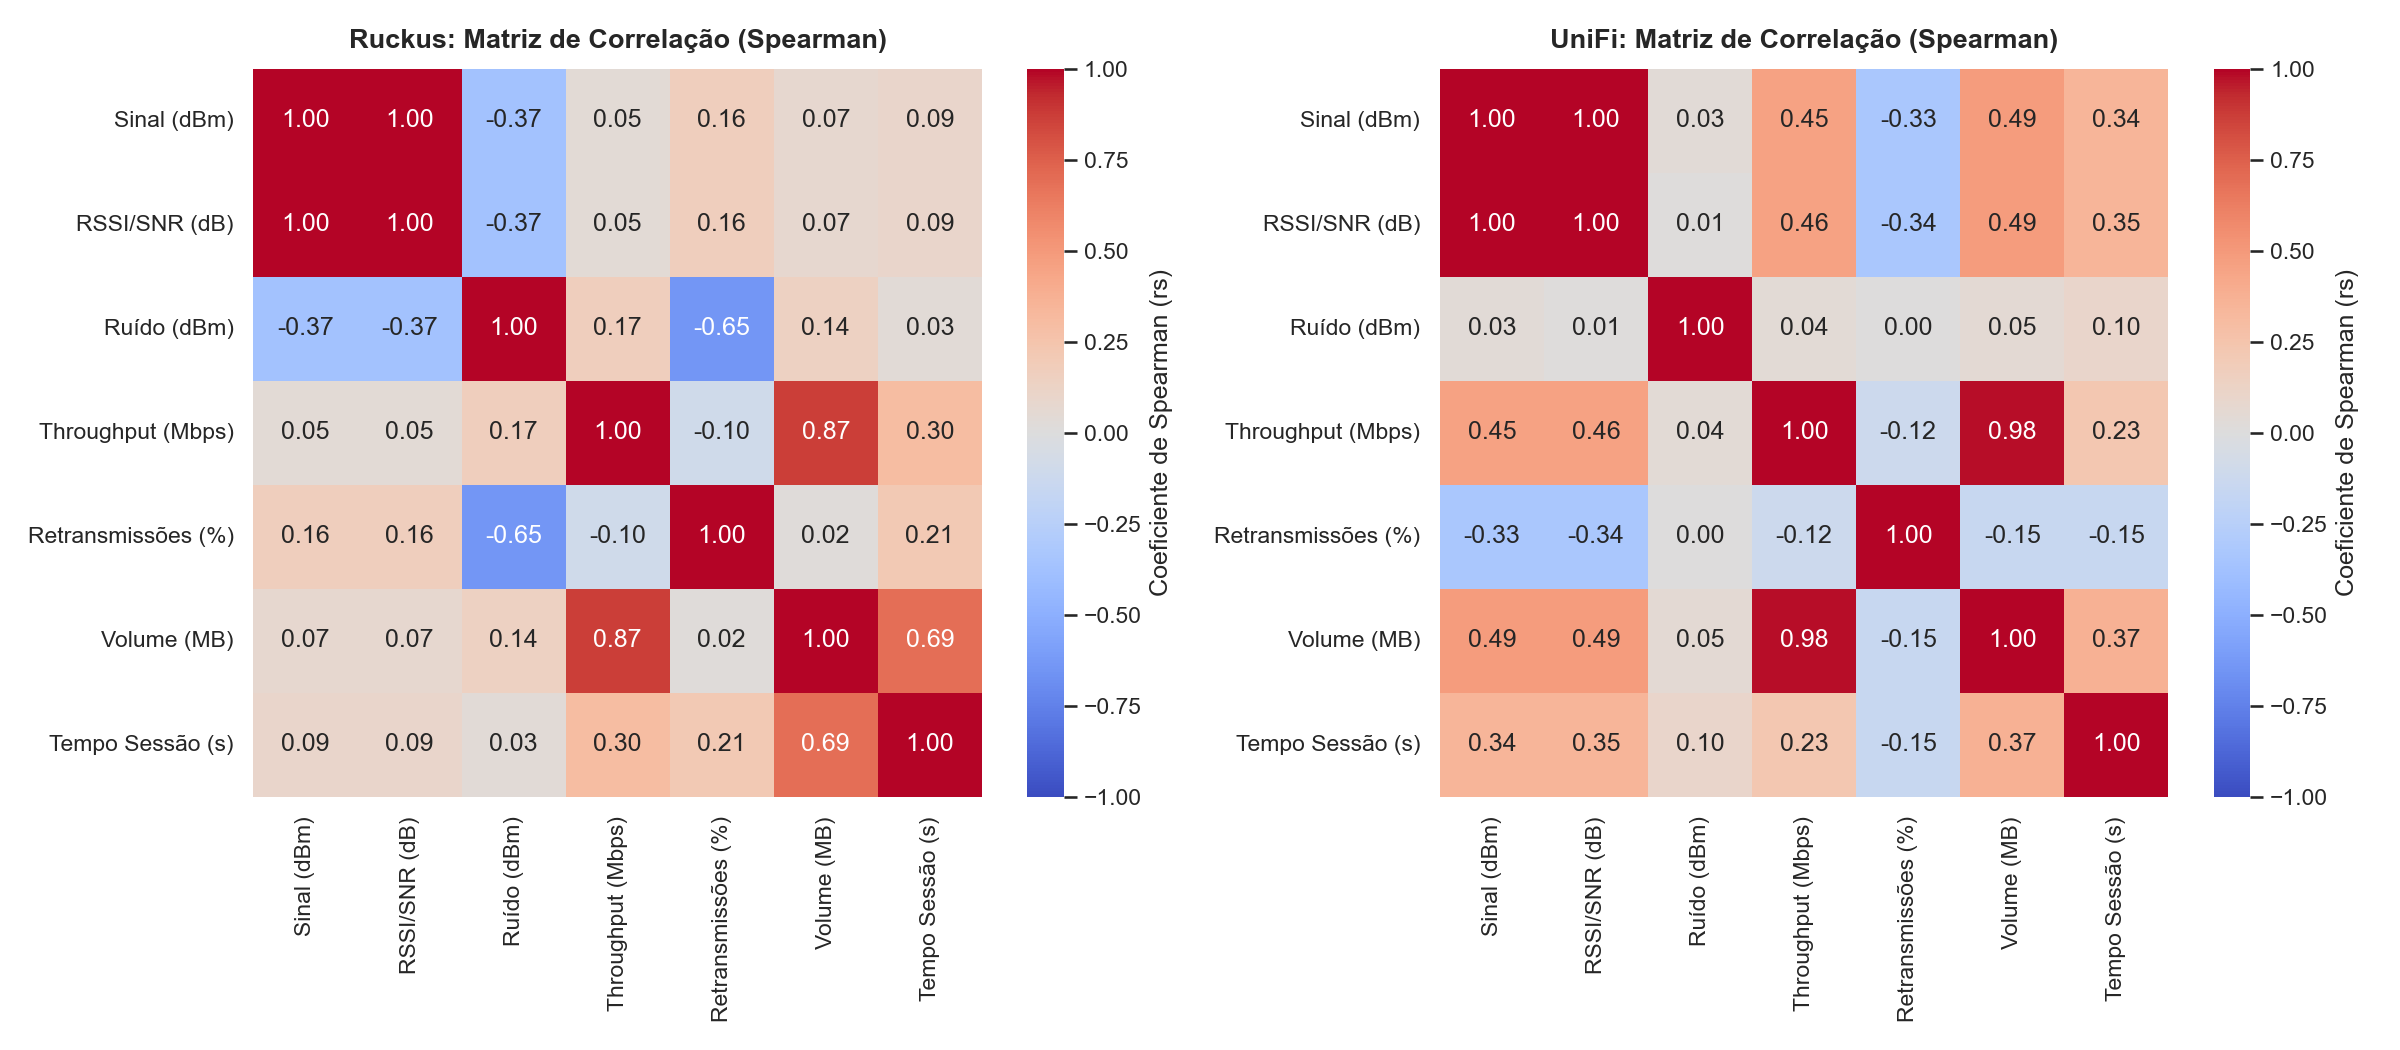
\includegraphics[width=0.85\textwidth]{img/matriz_correlacao_heatmap.png}
  \caption{Matriz de Correlação Heatmap}
  \label{fig:matriz_correlacao_heatmap_png}
\end{figure}

\begin{itemize}
  \item \textbf{Ruckus}: Exibe correlações monotônicas muito fortes entre Sinal e RSSI (sendo a mesma grandeza física mapeada) e o forte acoplamento linear artificial entre Ruído (Noise) e Sinal derivado do método de cálculo. O Throughput dos clientes individuais apresenta baixíssima correlação com a potência do sinal (\textit{r\_s} = 0.0363), condizente com o comportamento de ociosidade predominante.
  \item \textbf{UniFi}: O sinal absoluto (signal) e o RSSI (que atua como índice SNR) exibem correlação positiva moderada a forte (\textit{r\_s} = 0.70). O Throughput individual também apresenta correlação extremamente baixa com a intensidade de sinal (\textit{r\_s} = 0.4512). O ruído de fundo (noise) exibe baixíssima correlação com o sinal, validando a física do meio.
\end{itemize}


\subsection{Análise de Cada Gráfico de Dispersão}

\subsubsection{RSSI × Throughput}
\begin{itemize}
  \item \textbf{Arquivo}: `01\_rssi\_throughput.png`
  \item \textbf{Visualização}:
\end{itemize}
\begin{figure}[H]
  \centering
  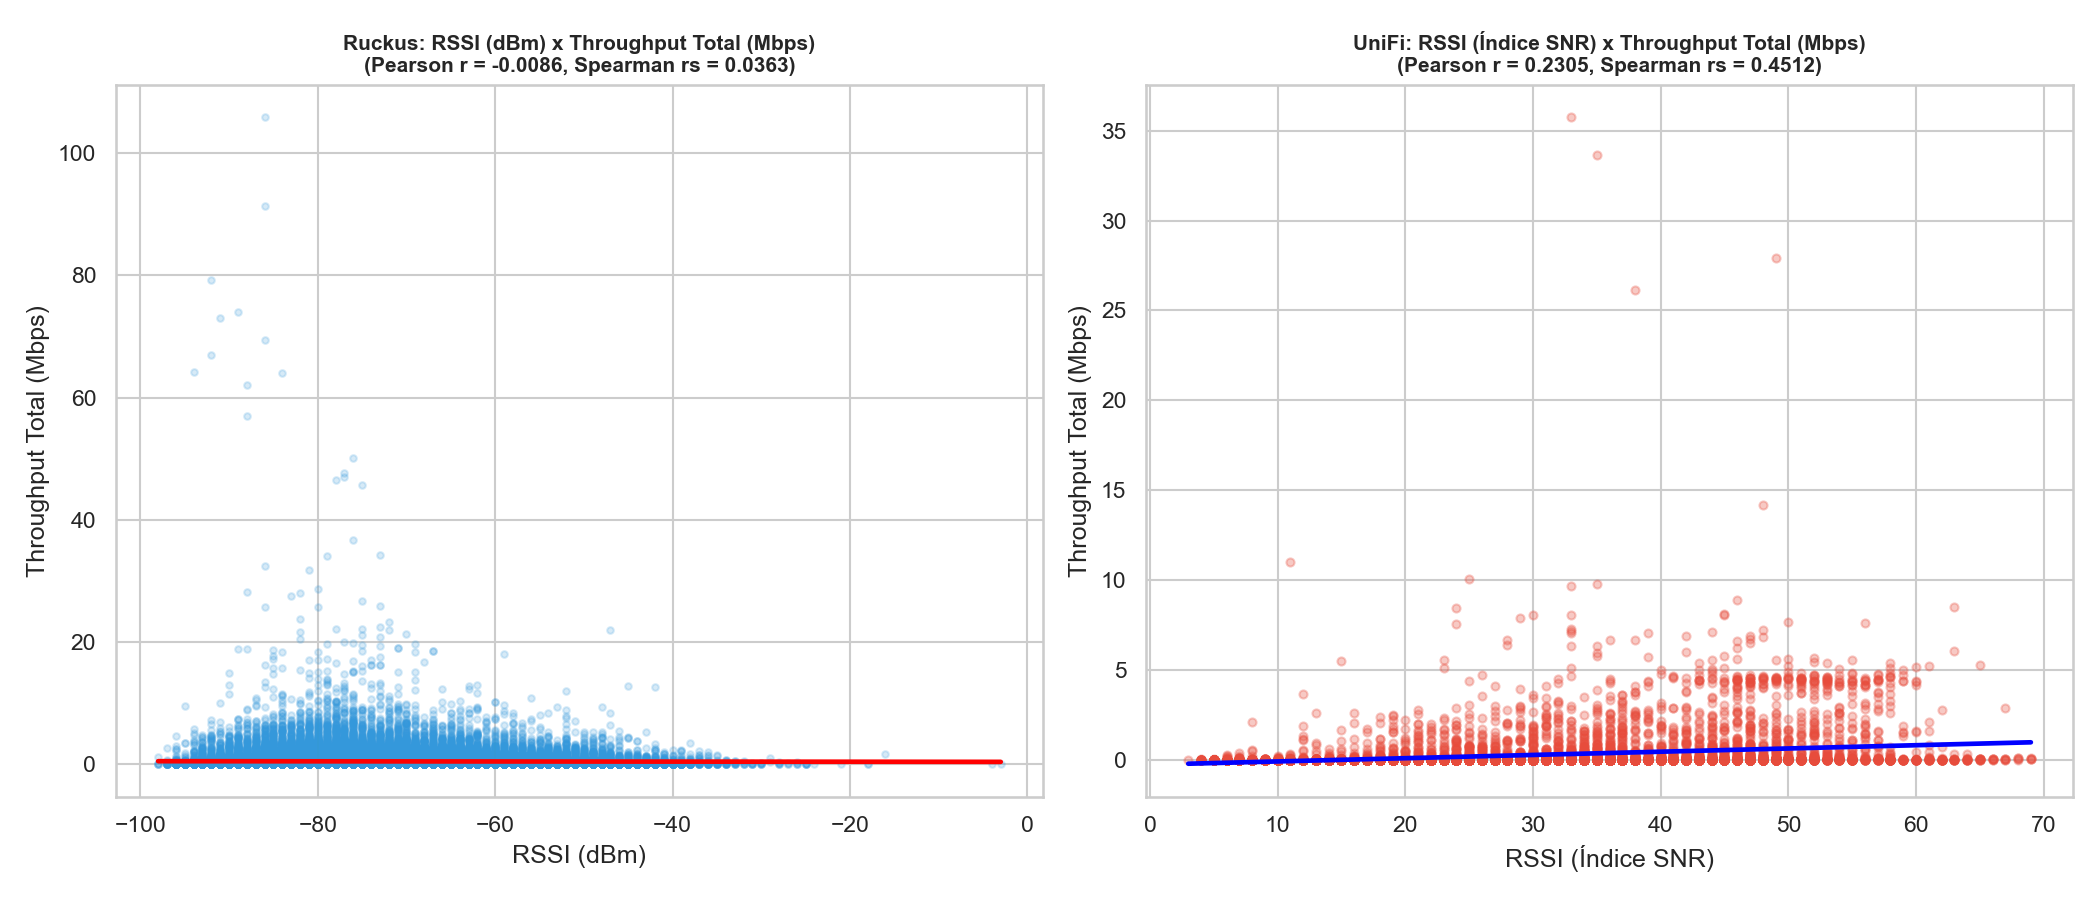
\includegraphics[width=0.85\textwidth]{img/01_rssi_throughput.png}
  \caption{RSSI x Throughput}
  \label{fig:01_rssi_throughput_png}
\end{figure}
\begin{itemize}
  \item \textbf{Expectativa Teórica}: Esperava-se uma correlação positiva moderada a forte. Sinais com melhor intensidade (RSSI alto) permitem modulações e taxas físicas maiores, o que deveria se traduzir em taxas mais altas de transferência ativa.
  \item \textbf{Comportamento Observado}: Os dados sugerem correlação praticamente nula no Ruckus (\textit{r\_p} = -0.0086, \textit{r\_s} = 0.0363) e fraca na UniFi (\textit{r\_p} = 0.2305, \textit{r\_s} = 0.4512).
  \item \textbf{Discussão}: Esta divergência sugere que o throughput de dados ativo depende fundamentalmente do padrão de demanda do usuário no instante de coleta. A maioria esmagadora dos dispositivos conectados permaneceu ociosa ou gerando tráfego insignificante (background sync), independentemente de estarem com sinal excelente ou intermediário.
\end{itemize}

\subsubsection{RSSI × Retransmissões}
\begin{itemize}
  \item \textbf{Arquivo}: `02\_rssi\_retransmissoes.png`
  \item \textbf{Visualização}:
\end{itemize}
\begin{figure}[H]
  \centering
  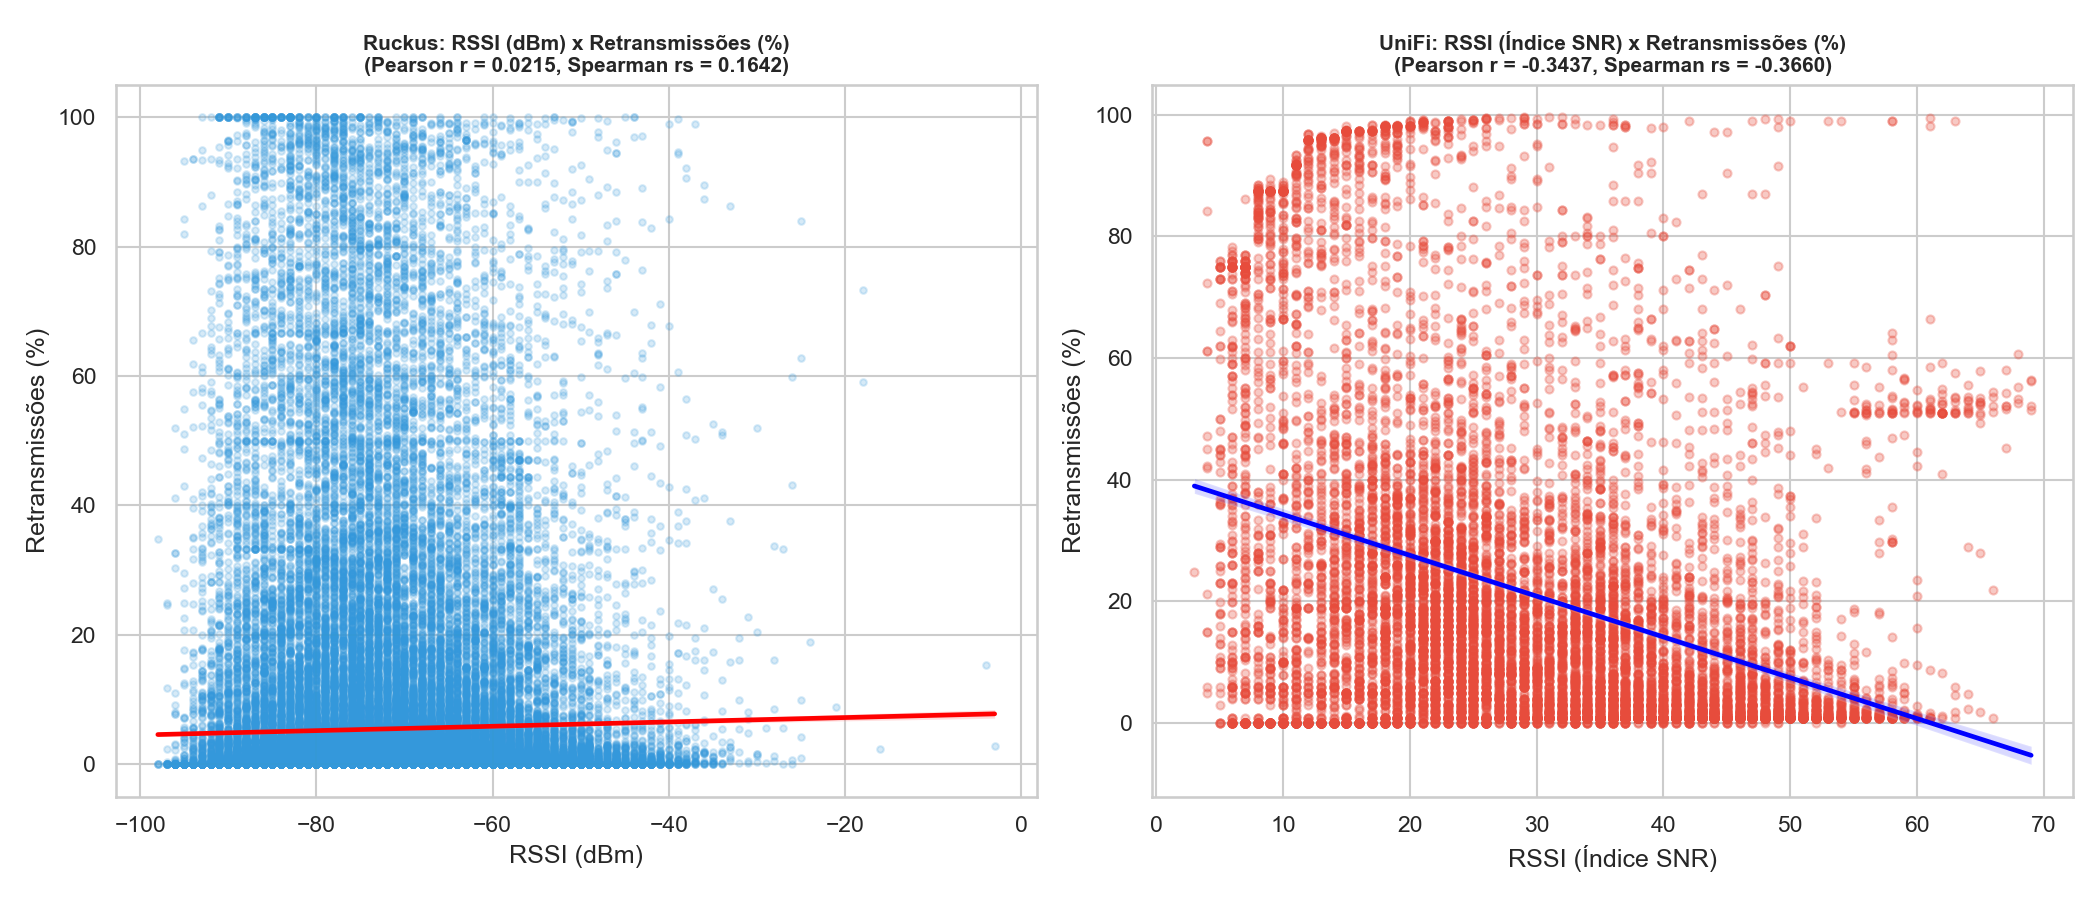
\includegraphics[width=0.85\textwidth]{img/02_rssi_retransmissoes.png}
  \caption{RSSI x Retransmissões}
  \label{fig:02_rssi_retransmissoes_png}
\end{figure}
\begin{itemize}
  \item \textbf{Expectativa Teórica}: Esperava-se uma correlação negativa moderada a forte. Níveis fracos de sinal costumam reduzir o SNR, elevando a taxa de bits incorretos (BER) e gerando retransmissões para recuperar os pacotes.
  \item \textbf{Comportamento Observado}: Correlação negativa muito fraca no Ruckus (\textit{r\_p} = 0.0215, \textit{r\_s} = 0.1642) e negativa moderada na UniFi (\textit{r\_p} = -0.3437, \textit{r\_s} = -0.3660).
  \item \textbf{Discussão}: Os dados da UniFi são consistentes com a teoria de que o sinal fraco prejudica o canal. Na Ruckus, a fraca correlação observada indica a atuação de mecanismos de hardware e software (como antenas inteligentes BeamFlex e controle de potência dinâmico) que evitam a perda excessiva de quadros físicos mesmo em níveis moderadamente baixos de sinal.
\end{itemize}

\subsubsection{Retransmissões × Throughput}
\begin{itemize}
  \item \textbf{Arquivo}: `03\_retransmissoes\_throughput.png`
  \item \textbf{Visualização}:
\end{itemize}
\begin{figure}[H]
  \centering
  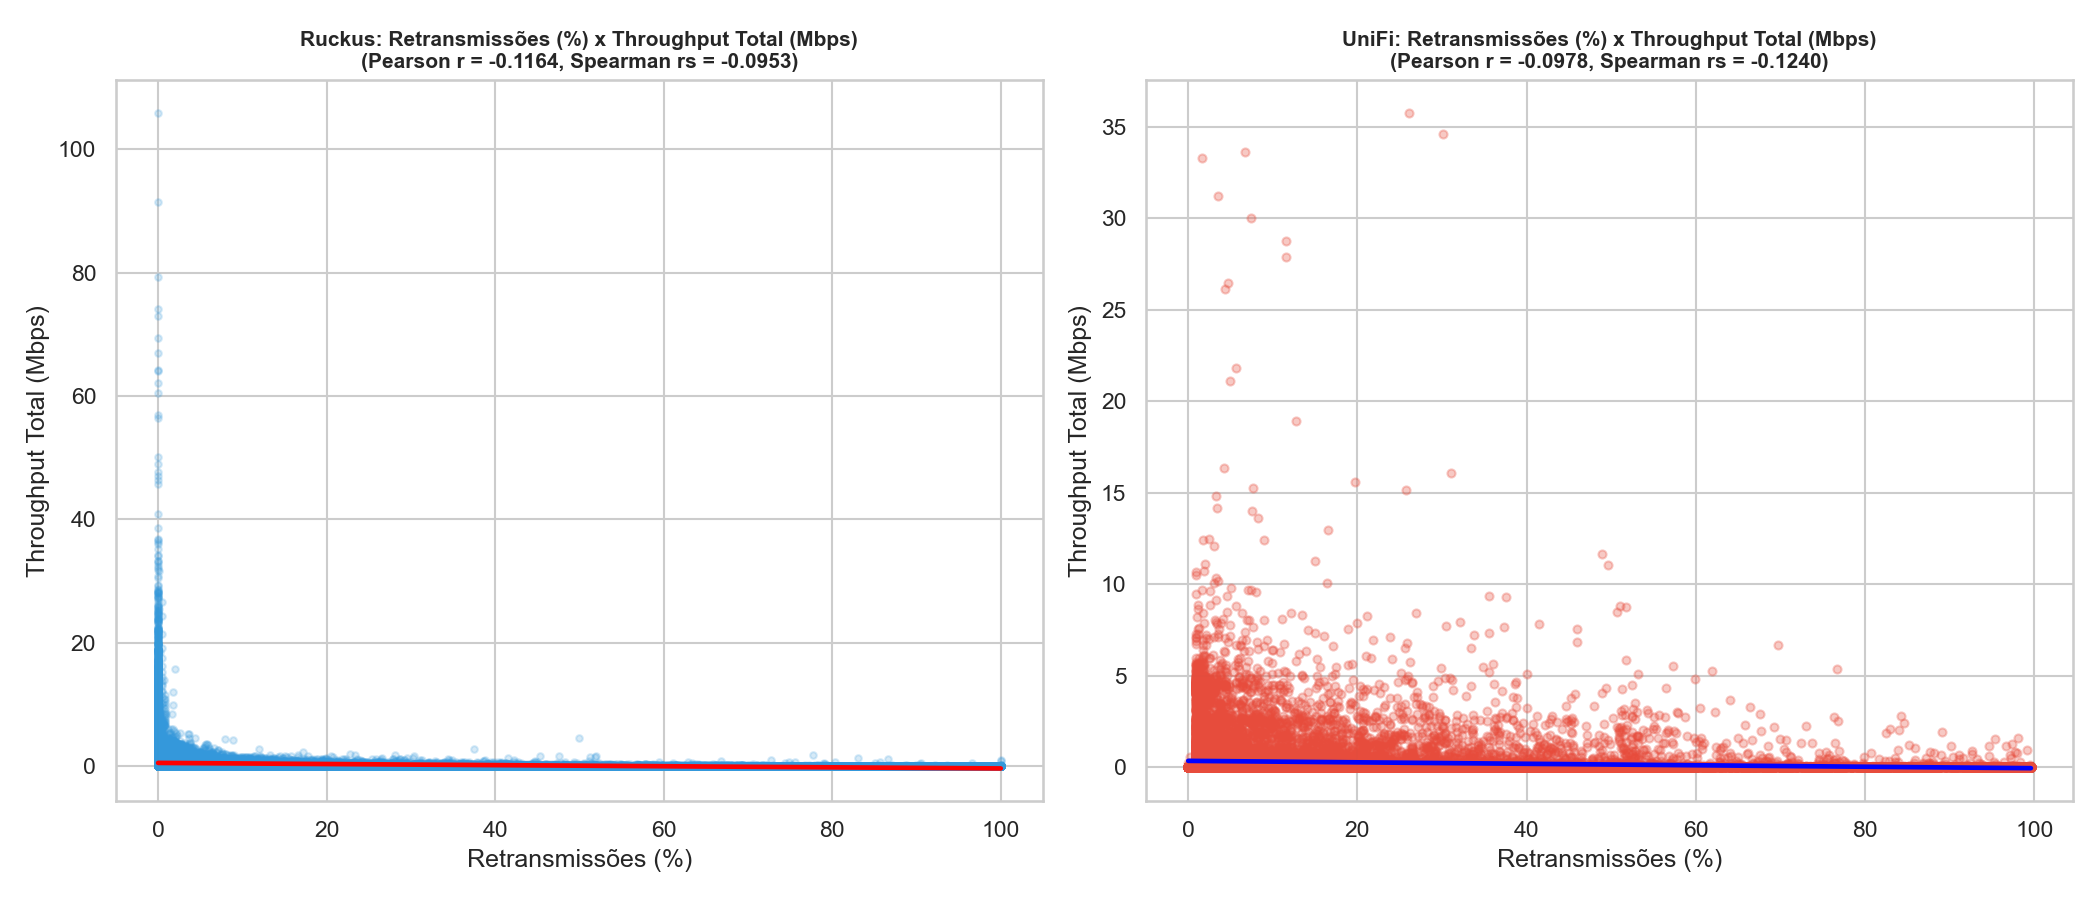
\includegraphics[width=0.85\textwidth]{img/03_retransmissoes_throughput.png}
  \caption{Retransmissões x Throughput}
  \label{fig:03_retransmissoes_throughput_png}
\end{figure}
\begin{itemize}
  \item \textbf{Expectativa Teórica}: Esperava-se uma correlação negativa moderada, pois altas retransmissões consomem tempo de canal de RF (airtime) e reduzem a capacidade útil.
  \item \textbf{Comportamento Observado}: Correlação negativa fraca no Ruckus (\textit{r\_p} = -0.1009, \textit{r\_s} = -0.0768) e na UniFi (\textit{r\_p} = -0.0989, \textit{r\_s} = -0.1321).
  \item \textbf{Discussão}: Os resultados sugerem que, como o throughput ativo na rede está muito longe do teto operacional dos canais (baixa carga ativa), o impacto de retransmissões dispersas no throughput do usuário não se mostrou severo o suficiente para gerar decréscimo drástico na taxa média registrada.
\end{itemize}

\subsubsection{Quantidade de Clientes × Throughput Agregado do AP}
\begin{itemize}
  \item \textbf{Arquivo}: `04\_clientes\_throughput\_ap.png`
  \item \textbf{Visualização}:
\end{itemize}
\begin{figure}[H]
  \centering
  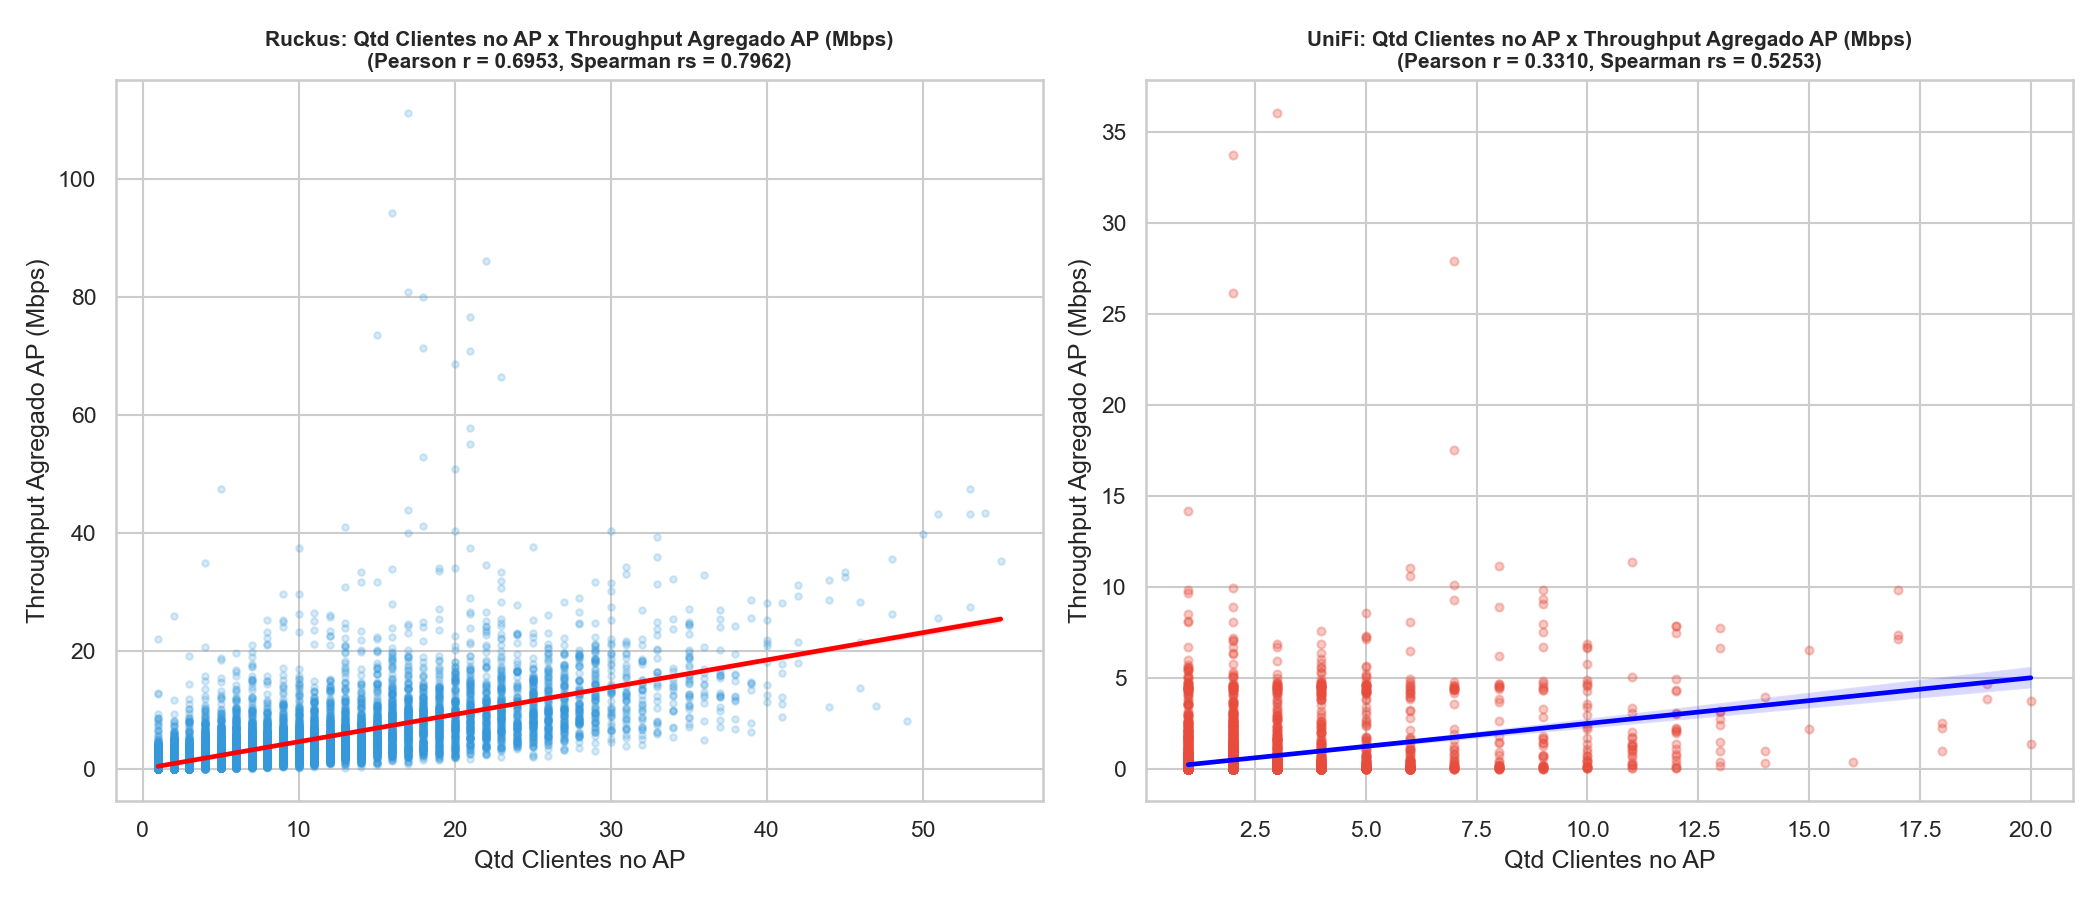
\includegraphics[width=0.85\textwidth]{img/04_clientes_throughput_ap.png}
  \caption{Clientes x Throughput Agregado}
  \label{fig:04_clientes_throughput_ap_png}
\end{figure}
\begin{itemize}
  \item \textbf{Expectativa Teórica}: Esperava-se uma correlação positiva moderada a forte, visto que o tráfego total somado em um AP tende a crescer proporcionalmente com a quantidade de dispositivos ativos gerando tráfego concorrente.
  \item \textbf{Comportamento Observado}: Os dados indicam correlação positiva forte no Ruckus (\textit{r\_p} = 0.6953, \textit{r\_s} = 0.7962) e positiva moderada a forte na UniFi (\textit{r\_p} = 0.3310, \textit{r\_s} = 0.5253).
  \item \textbf{Discussão}: Esse resultado é consistente com o esperado teoricamente. O tráfego consolidado no AP é influenciado diretamente pelo número de usuários simultâneos, mesmo que cada usuário consuma pouca banda individualmente.
\end{itemize}

\subsubsection{Quantidade de Clientes × Retransmissões Médias do AP}
\begin{itemize}
  \item \textbf{Arquivo}: `05\_clientes\_retransmissoes\_ap.png`
  \item \textbf{Visualização}:
\end{itemize}
\begin{figure}[H]
  \centering
  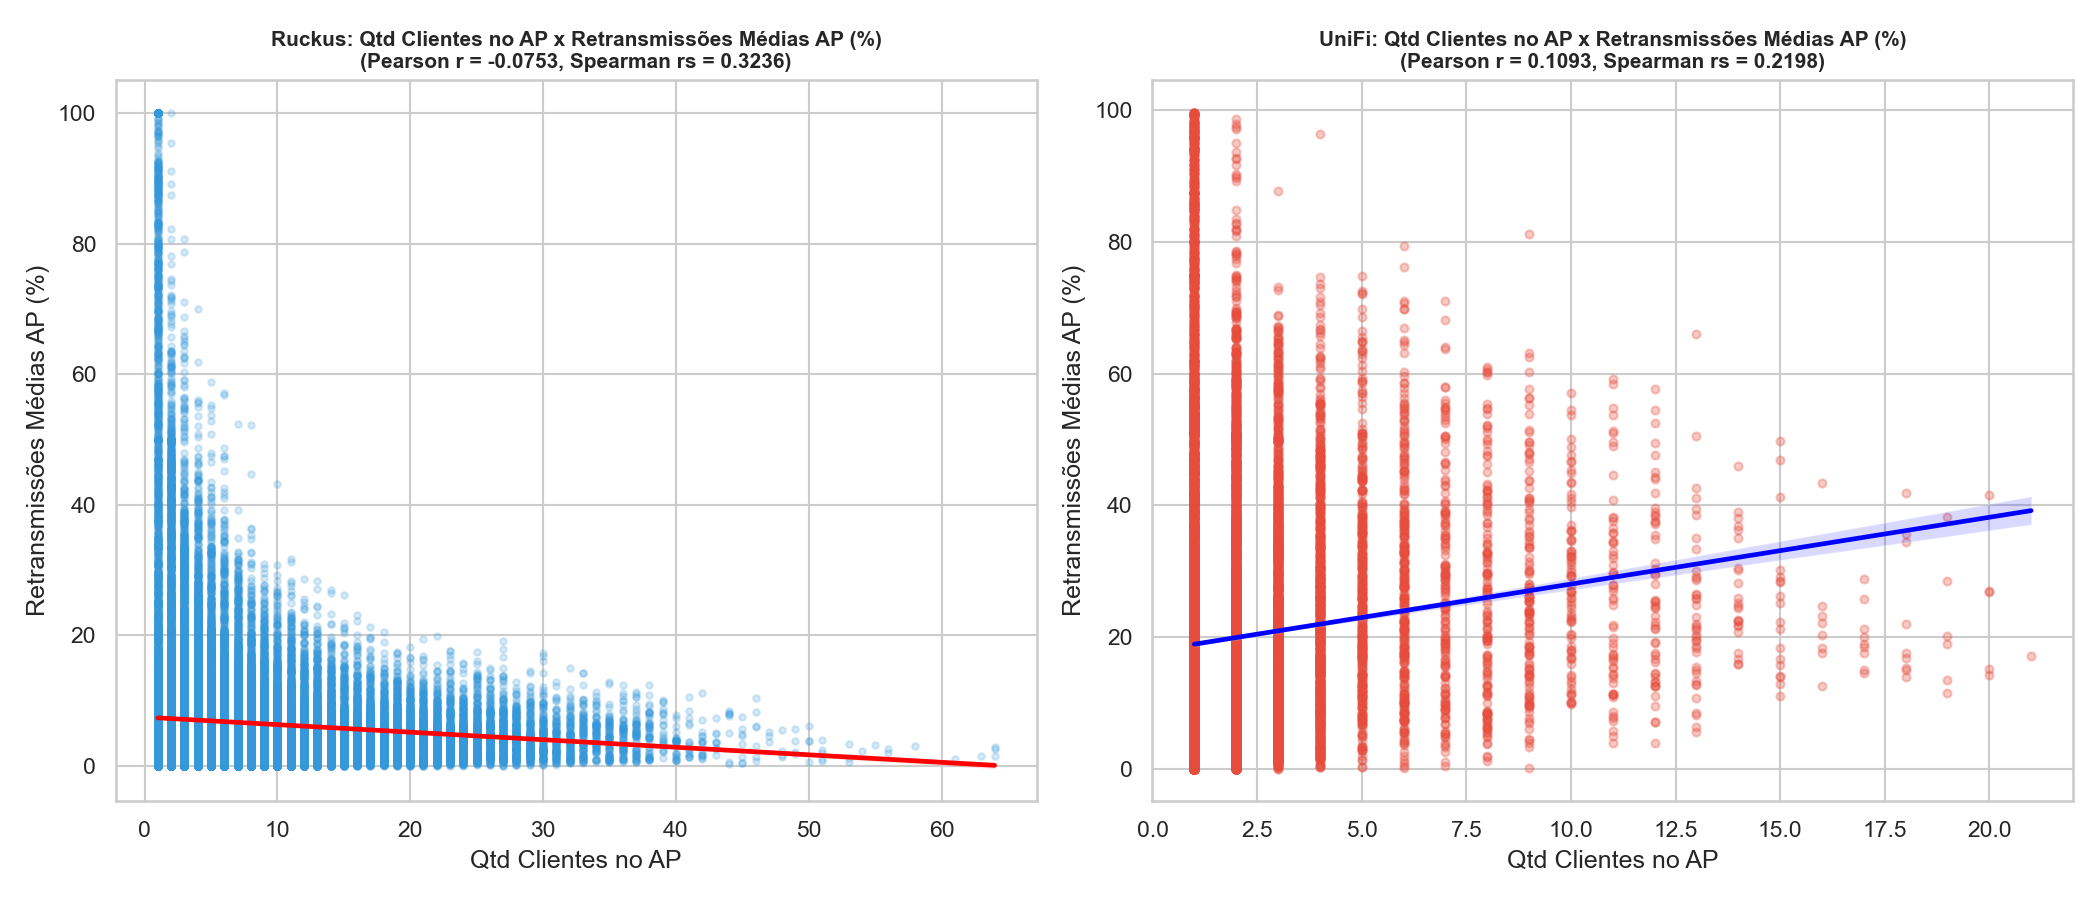
\includegraphics[width=0.85\textwidth]{img/05_clientes_retransmissoes_ap.png}
  \caption{Clientes x Retransmissões AP}
  \label{fig:05_clientes_retransmissoes_ap_png}
\end{figure}
\begin{itemize}
  \item \textbf{Expectativa Teórica}: Esperava-se uma correlação positiva moderada, dado que mais clientes compartilhando o canal físico via protocolo CSMA/CA aumentam as chances de colisão no ar.
  \item \textbf{Comportamento Observado}: Os dados mostram correlação nula no Ruckus (\textit{r\_p} = -0.0590, \textit{r\_s} = 0.3572) e muito fraca na UniFi (\textit{r\_p} = 0.1081, \textit{r\_s} = 0.2302).
  \item \textbf{Discussão}: Os coeficientes sugerem que os APs de ambas as marcas conseguem lidar satisfatoriamente com a coordenação de pacotes dos clientes e evitar colisões críticas sob as cargas observadas durante a coleta.
\end{itemize}

\subsubsection{Ruído de Fundo (Noise) × Retransmissões}
\begin{itemize}
  \item \textbf{Arquivo}: `06\_noise\_retransmissoes.png`
  \item \textbf{Visualização}:
\end{itemize}
\begin{figure}[H]
  \centering
  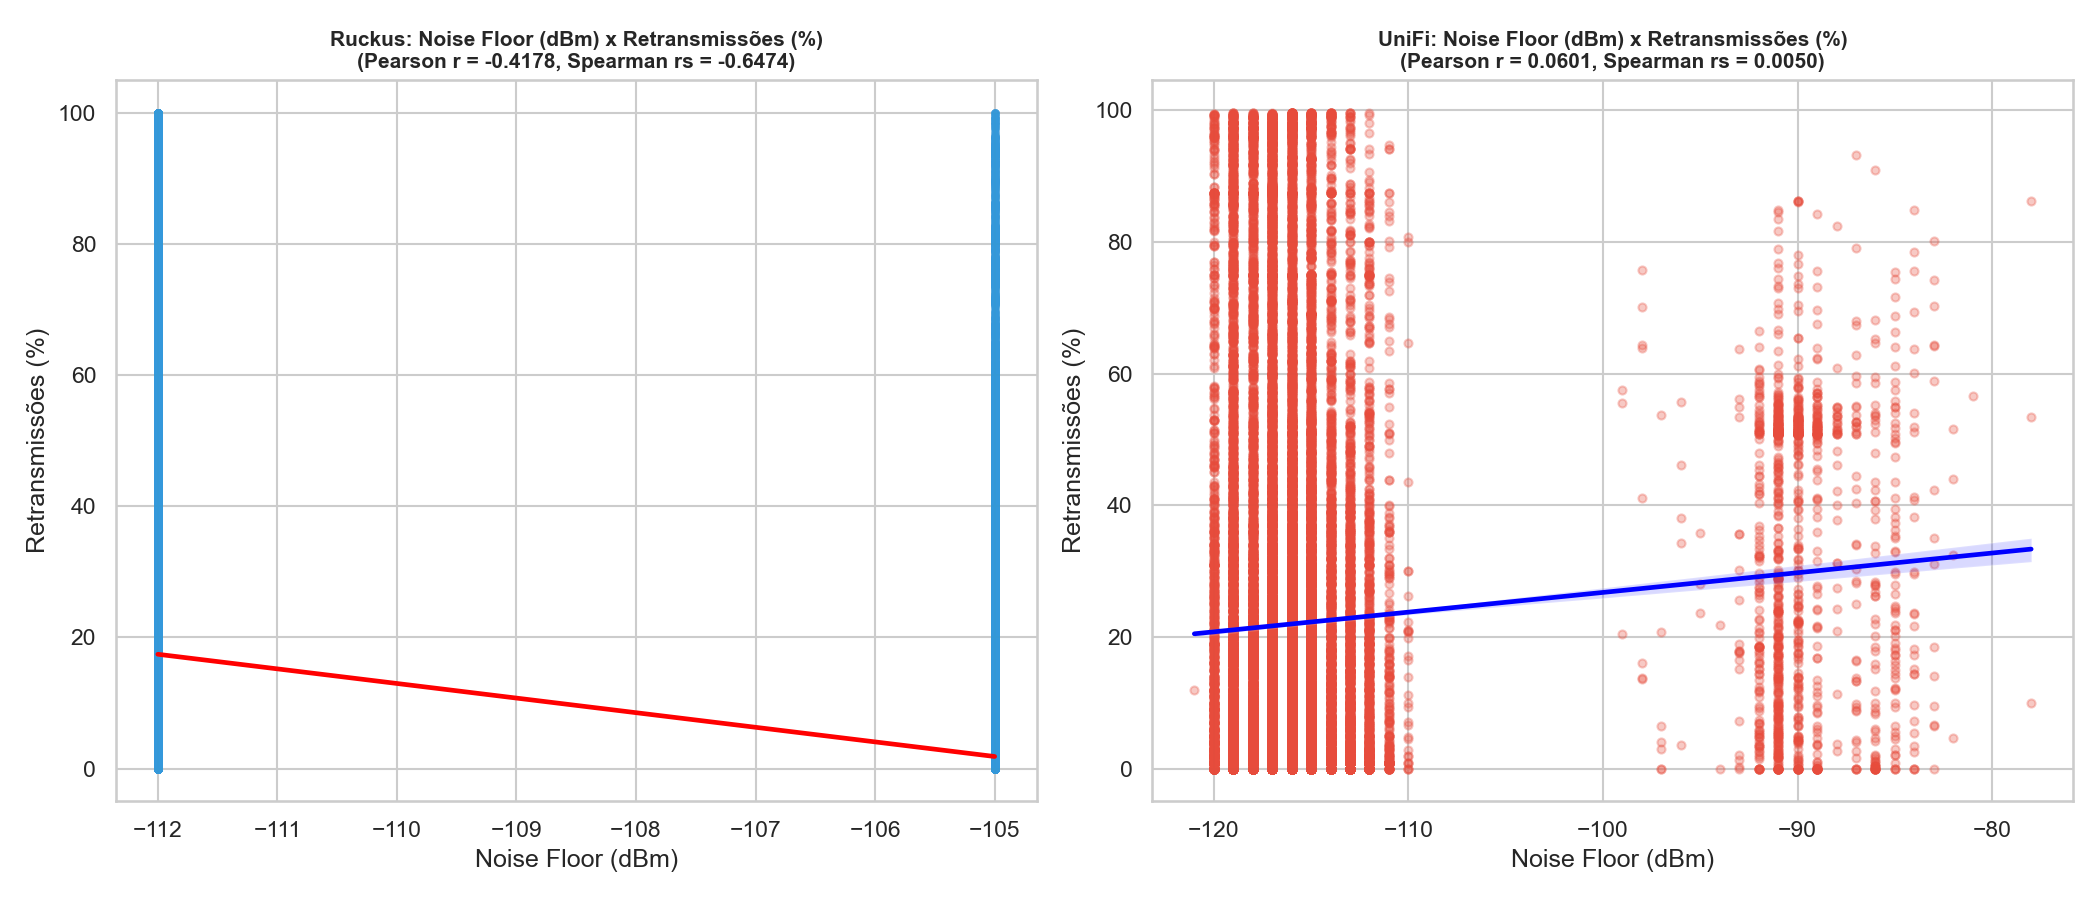
\includegraphics[width=0.85\textwidth]{img/06_noise_retransmissoes.png}
  \caption{Noise x Retransmissões}
  \label{fig:06_noise_retransmissoes_png}
\end{figure}
\begin{itemize}
  \item \textbf{Expectativa Teórica}: Esperava-se correlação positiva, uma vez que níveis de ruído elevados deterioram o SNR e a integridade física dos bits transmitidos.
  \item \textbf{Comportamento Observado}: Correlação nula no Ruckus (\textit{r\_p} = -0.3952, \textit{r\_s} = -0.6323) e na UniFi (\textit{r\_p} = 0.0447, \textit{r\_s} = -0.0043).
  \item \textbf{Discussão}: Isso sugere que o ruído ambiental no campus permaneceu em patamares baixos e estáveis (sem picos severos de interferência externa), não afetando de forma mensurável a estabilidade de pacotes nas conexões dos clientes.
\end{itemize}

\subsubsection{Ruído de Fundo (Noise) × RSSI}
\begin{itemize}
  \item \textbf{Arquivo}: `07\_noise\_rssi.png`
  \item \textbf{Visualização}:
\end{itemize}
\begin{figure}[H]
  \centering
  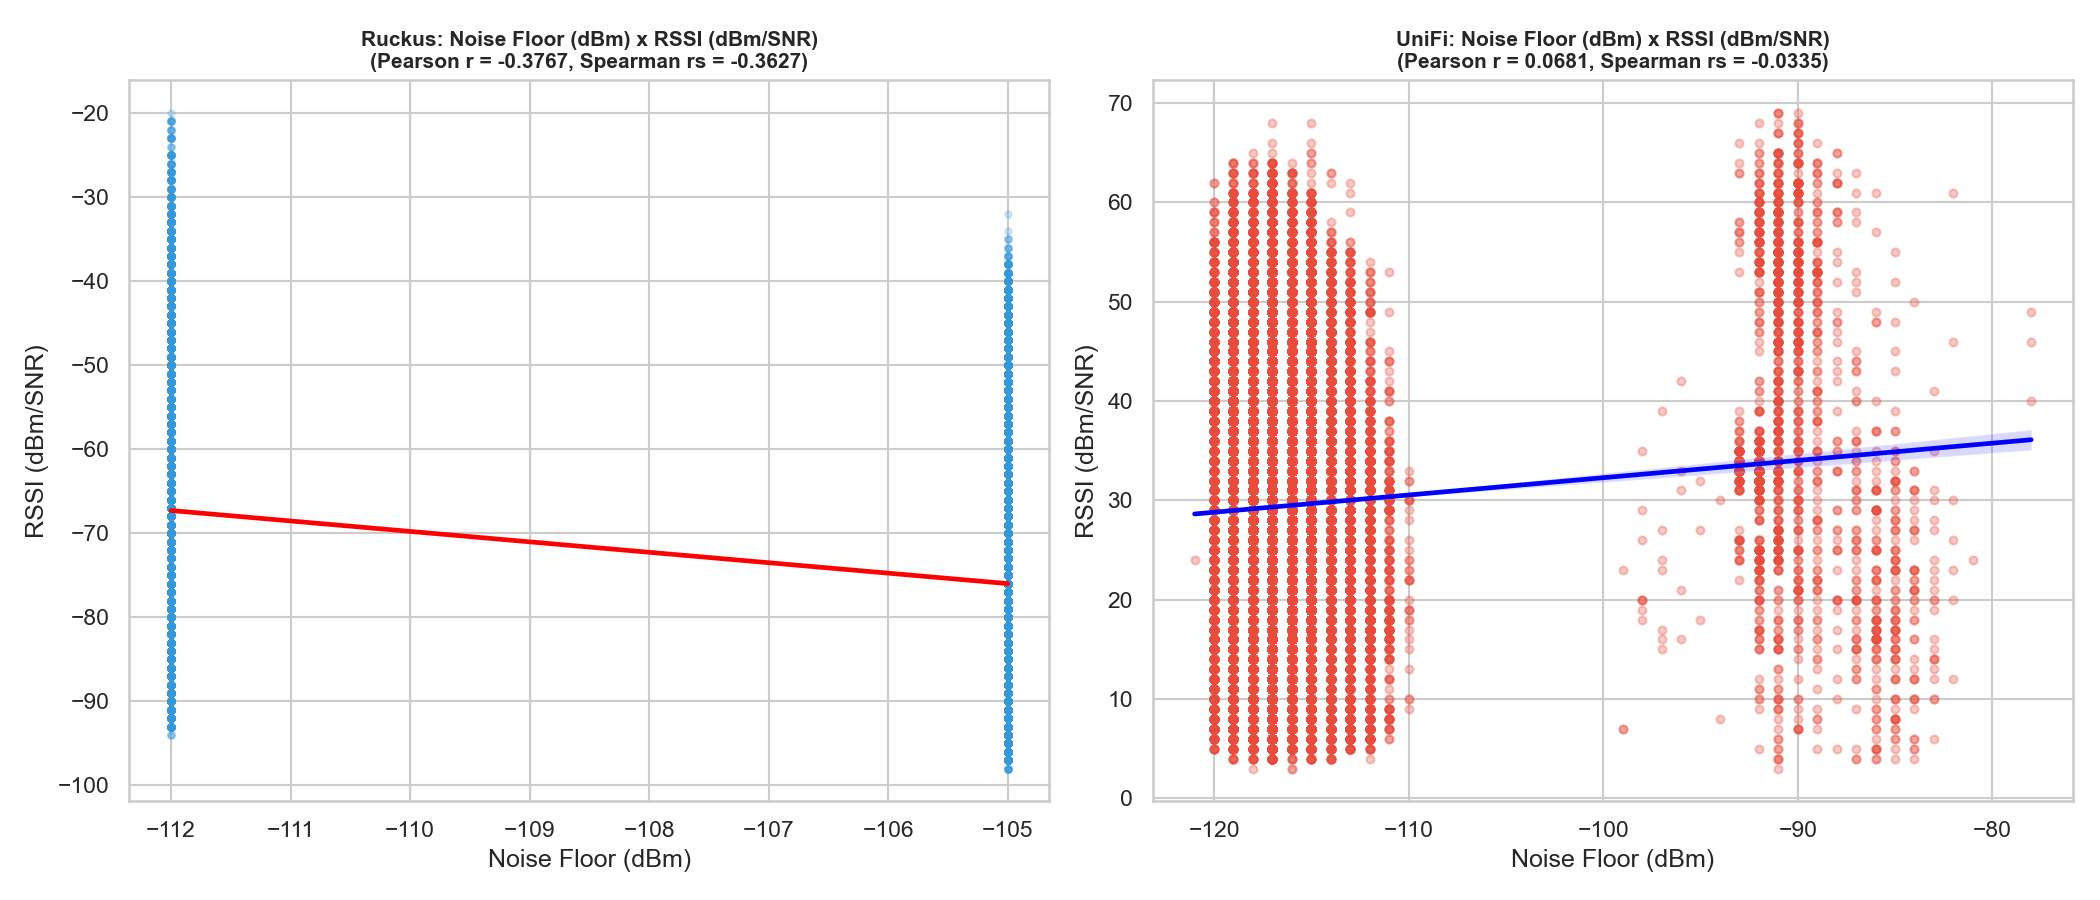
\includegraphics[width=0.85\textwidth]{img/07_noise_rssi.png}
  \caption{Noise x RSSI}
  \label{fig:07_noise_rssi_png}
\end{figure}
\begin{itemize}
  \item \textbf{Expectativa Teórica}: Esperava-se correlação nula. Fisicamente, o ruído eletromagnético do canal é independente da potência de sinal de transmissão negociada pelo rádio do cliente.
  \item \textbf{Comportamento Observado}: Correlação nula na UniFi (\textit{r\_p} = 0.1053, \textit{r\_s} = 0.0083), mas muito forte na Ruckus (\textit{r\_p} = -0.3933, \textit{r\_s} = -0.3762).
  \item \textbf{Discussão}: O resultado da UniFi apóia a física do canal de rádio. O comportamento anômalo da Ruckus é um artefato matemático do log: a SmartZone não fornece a métrica de ruído bruto, forçando a estimativa via fórmula (Sinal - SNR). Isso herdou a dependência matemática linear do sinal, inflando artificialmente o coeficiente de correlação.
\end{itemize}

\subsubsection{Link Speed TX × Throughput TX}
\begin{itemize}
  \item \textbf{Arquivo}: `08\_link\_speed\_throughput.png`
  \item \textbf{Visualização}:
\end{itemize}
\begin{figure}[H]
  \centering
  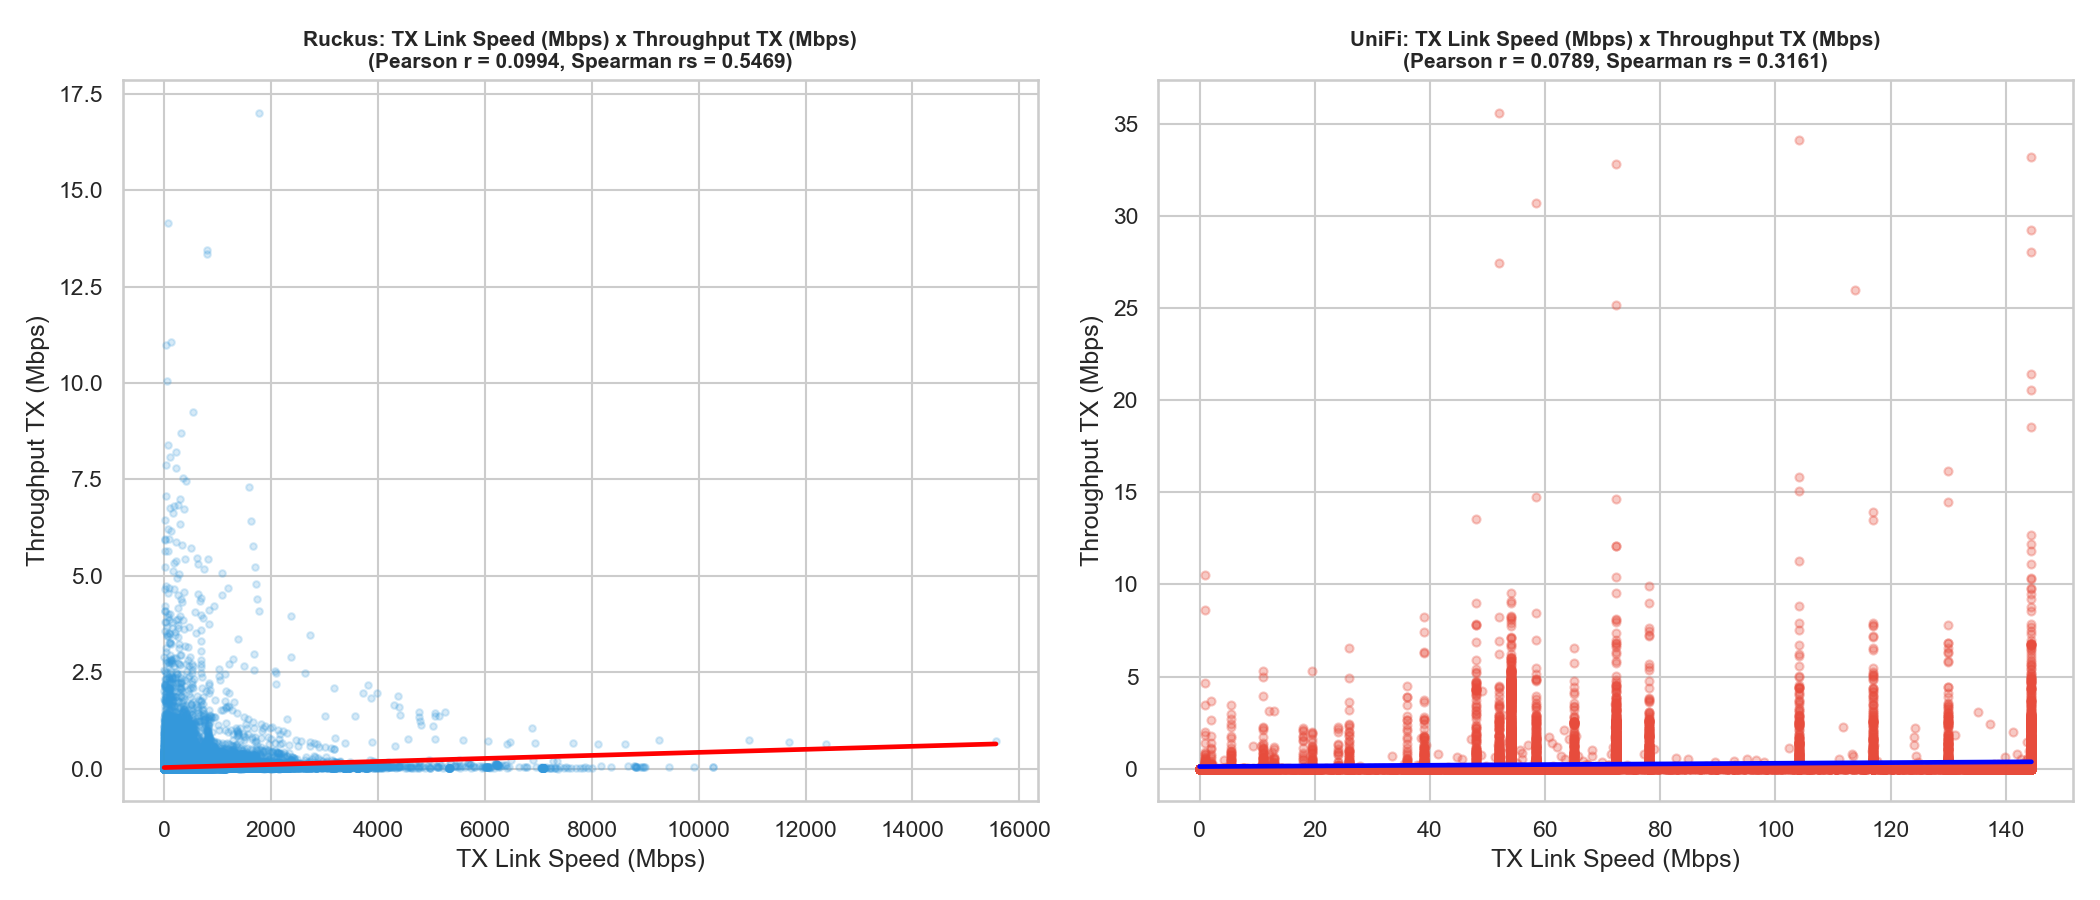
\includegraphics[width=0.85\textwidth]{img/08_link_speed_throughput.png}
  \caption{Link Speed x Throughput}
  \label{fig:08_link_speed_throughput_png}
\end{figure}
\begin{itemize}
  \item \textbf{Expectativa Teórica}: Esperava-se uma correlação positiva moderada. Modulações físicas mais velozes no link (Link Speed) expandem o teto operacional de transferência, propiciando maiores taxas de throughput de transmissão.
  \item \textbf{Comportamento Observado}: Correlação fraca no Ruckus (\textit{r\_p} = 0.1086, \textit{r\_s} = 0.5475) e nula na UniFi (\textit{r\_p} = 0.0536, \textit{r\_s} = 0.2877).
  \item \textbf{Discussão}: Esse resultado indica que a modulação de velocidade do link de rádio é mantida elevada pela proximidade física, porém a vazão real consumida depende exclusivamente do perfil e uso de aplicativos pelo cliente.
\end{itemize}

\subsubsection{Volume de Dados × Tempo de Sessão (Uptime)}
\begin{itemize}
  \item \textbf{Arquivo}: `09\_ruckus\_uptime\_volume.png`
  \item \textbf{Visualização}:
\end{itemize}
\begin{figure}[H]
  \centering
  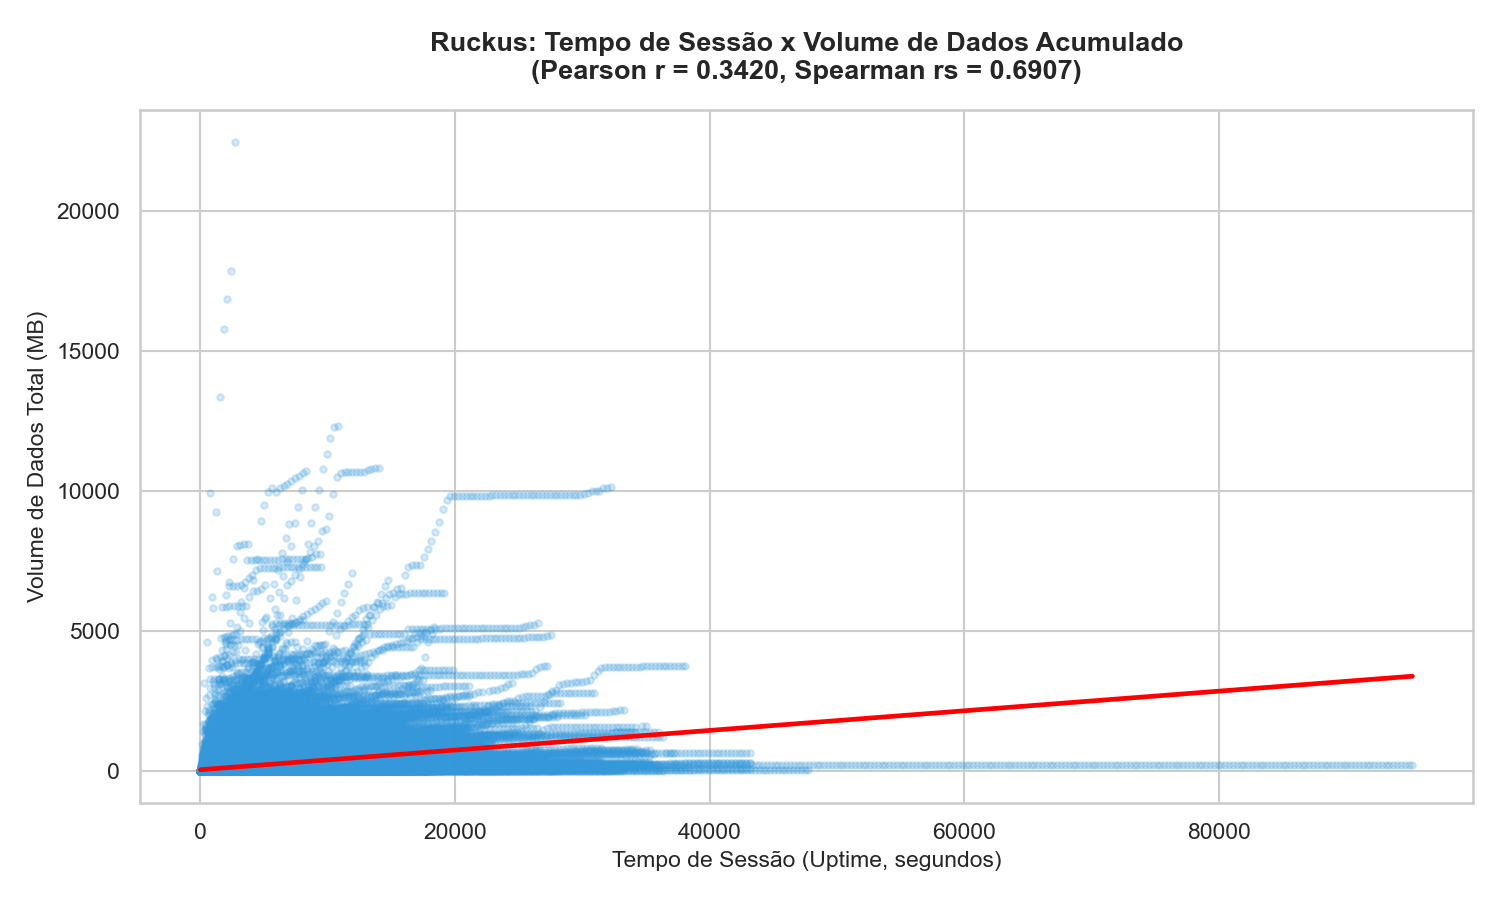
\includegraphics[width=0.85\textwidth]{img/09_ruckus_uptime_volume.png}
  \caption{Tempo de Sessão x Volume Ruckus}
  \label{fig:09_ruckus_uptime_volume_png}
\end{figure}
\begin{itemize}
  \item \textbf{Expectativa Teórica}: Esperava-se uma correlação positiva moderada a forte, dado que sessões de conexão mais duradouras propiciam o acúmulo integrado de mais bytes trafegados.
  \item \textbf{Comportamento Observado}: Correlação positiva moderada a forte no Ruckus (\textit{r\_p} = 0.3417, \textit{r\_s} = 0.6861) e na UniFi (\textit{r\_p} = 0.0980, \textit{r\_s} = 0.3121).
  \item \textbf{Discussão}: Os dados são consistentes com a teoria de rede. Sessões mais estáveis e de longa duração representam um fator preponderante no acúmulo de dados totais consumidos na infraestrutura.
\end{itemize}

